
\chapter{Preliminary Preparation}
\label{ch:prelim}

This chapter presents the preliminary experimental work undertaken to
verify that a lightweight, container-based platform can exhibit the
capacity-planning phenomena targeted by this thesis. The goals of these
experiments were to:

\begin{enumerate}
    \item confirm that a single Dockerised microservice shows measurable
    changes in latency and tail behaviour under varying request rates;
    \item validate that standard observability tools can capture traces
    suitable for parameterising queueing and simulation models; and
    \item assess whether the resulting behaviour aligns with the
    capacity-planning challenges outlined in Chapter~\ref{ch:litreview},
    namely saturation, tail-latency growth, and resource contention.
\end{enumerate}

The results in this chapter form the empirical foundation for the
hybrid ML--DES modelling framework developed in later chapters.

%-------------------------------------------------------------
\section{Experimental Environment}
\label{sec:prelim-env}

\subsection{Microservice and Container Configuration}

The system under test is a simple HTTP microservice deployed as a Docker
container. The service is based on a lightweight echo-style server
(`http-echo`), chosen to minimise application-level complexity so that
observed performance effects predominantly arise from CPU contention and
scheduling rather than business logic.

The container is configured with:
\begin{itemize}
    \item a single virtual CPU (Docker CPU quota of 1.0);
    \item minimal memory allocation (sufficient to avoid swapping); and
    \item a fixed request handler that performs a small, CPU-bound task
    before returning an HTTP~200 response.
\end{itemize}

This configuration makes the service effectively CPU-bound, ensuring
that increased load translates into contention for the single core.

\subsection{Load Generation with Vegeta}

Open-loop load generation is provided by \texttt{Vegeta}. For each
experiment, Vegeta issues HTTP~GET requests at a fixed rate~$\lambda$
for a duration of $60$~seconds. Three arrival rates were tested:

\begin{itemize}
    \item $\lambda = 800$~req/s,
    \item $\lambda = 1200$~req/s,
    \item $\lambda = 1600$~req/s.
\end{itemize}

These rates were chosen to exercise three operating regions:

\begin{enumerate}
    \item a sub-saturation region (800~req/s),
    \item a near-saturation region (1200~req/s),
    \item an overloaded region (1600~req/s).
\end{enumerate}

It is worth noting that Vegeta reports end-to-end response time rather than pure service time. The latter excludes queueing delay and cannot be observed directly from the client side. In this thesis, service-time distributions will be obtained in two stages (developed in Thesis~B). First, a baseline experiment will be run at a very low arrival rate, where queueing delay is negligible; in this regime the observed latencies are treated as samples from the underlying service-time distribution, from which an empirical shape (e.g.\ histogram or kernel density estimate) is derived. Second, for each workload and CPU-quota configuration, container CPU usage and throughput will be collected via cAdvisor/Prometheus and the mean service demand $S$ will be estimated using the Utilisation Law $U = X S$. The baseline distribution is then re-parameterised so that its mean matches the estimated $S$, or, equivalently, a machine-learning model learns a mapping from resource configuration and load to distribution parameters. These reconstructed service-time distributions will be used to calibrate the DES model, whereas this chapter presents only the measured response-time distributions.
Vegeta reports per-run statistics including mean latency, quantiles
(p50, p90, p95, p99), and maximum latency, which are used directly in
the analysis below.

\subsection{Observability Stack}

Although this chapter focuses on latency results, the experiments were
run within the full observability stack used throughout the thesis:

\begin{itemize}
    \item \textbf{cAdvisor} for per-container CPU utilisation and
    throttling metrics;
    \item \textbf{Prometheus} for scraping and storing time-series data;
    \item \textbf{Grafana} for visualising utilisation and latency.
\end{itemize}

These tools confirm that the service is CPU-bound and that the container
approaches 100\% CPU usage in the high-load regime, but the numerical
CPU traces are omitted here for brevity. The key latency statistics are
summarised in the following section.

%-------------------------------------------------------------
\section{Load-Test Results}
\label{sec:prelim-results}

\subsection{Latency Summary}

Table~\ref{tab:vegeta-latency} summarises the Vegeta results for the
three fixed request rates. Each run lasted 60~seconds and achieved a
100\% success rate (no HTTP errors).

\begin{table}[h]
\centering
\caption{Latency measurements for the Dockerised microservice under
different request rates (Vegeta, 60~s runs).}
\label{tab:vegeta-latency}
\begin{tabular}{rrrrrrrrr}
\toprule
\multicolumn{1}{c}{$\lambda$} &
\multicolumn{1}{c}{Total} &
\multicolumn{1}{c}{Mean} &
\multicolumn{1}{c}{p50} &
\multicolumn{1}{c}{p90} &
\multicolumn{1}{c}{p95} &
\multicolumn{1}{c}{p99} &
\multicolumn{1}{c}{Max} &
\multicolumn{1}{c}{Success} \\
\multicolumn{1}{c}{(req/s)} &
\multicolumn{1}{c}{requests} &
\multicolumn{1}{c}{(ms)} &
\multicolumn{1}{c}{(ms)} &
\multicolumn{1}{c}{(ms)} &
\multicolumn{1}{c}{(ms)} &
\multicolumn{1}{c}{(ms)} &
\multicolumn{1}{c}{(ms)} &
\multicolumn{1}{c}{(\%)} \\
\midrule
 800  & 48{,}000 & 1.185 & 1.097 & 1.325 & 1.490 &  2.528 & 26.849 & 100 \\
1200  & 72{,}000 & 1.287 & 1.159 & 1.480 & 1.648 &  4.223 & 24.758 & 100 \\
1600  & 96{,}000 & 1.518 & 1.236 & 1.583 & 1.860 &  6.959 & 93.737 & 100 \\
\bottomrule
\end{tabular}
\end{table}

For convenience, Table~\ref{tab:vegeta-mean-p99} extracts the mean,
p99, and maximum latencies---the metrics most relevant for capacity
planning and tail-behaviour analysis.

\begin{table}[h]
\centering
\caption{Mean, p99, and maximum latency as a function of request rate.}
\label{tab:vegeta-mean-p99}
\begin{tabular}{rrrr}
\toprule
$\lambda$ (req/s) & Mean (ms) & p99 (ms) & Max (ms) \\
\midrule
 800  & 1.185 & 2.528 & 26.849 \\
1200  & 1.287 & 4.223 & 24.758 \\
1600  & 1.518 & 6.959 & 93.737 \\
\bottomrule
\end{tabular}
\end{table}

Two patterns are immediately visible:

\begin{enumerate}
    \item the mean latency increases modestly with load, remaining below
    2~ms even at 1600~req/s; and
    \item the p99 and maximum latencies grow much more sharply, with
    p99 more than doubling between 800 and 1600~req/s, and the maximum
    latency reaching almost 94~ms at the highest rate.
\end{enumerate}

This separation between the behaviour of typical requests (mean, p50) and rare, slow requests (p99, max) is consistent with observations in production microservices, where high-percentile latencies are disproportionately affected by queueing delays, resource contention, and scheduling effects \cite{DeanBarroso2013}. The CPU utilisation plots obtained from cAdvisor clearly show the transition from stable operation to saturation. At 800~req/s, total CPU usage hovered below one core with balanced per-core activity, indicating that the service operated comfortably within capacity. At 1200~req/s, utilisation rose consistently and approached the single-core limit, but remained stable. At 1600~req/s, both total usage and per-core usage plateaued at the maximum available CPU allocation, demonstrating hard CPU saturation under high load.

This plateau corresponds directly to the rapid growth of the p99 and maximum latency observed in the Vegeta reports. The consistency between cAdvisor’s CPU traces and the sharp expansion of tail latencies supports the interpretation that the bottleneck is CPU-bound, validating the use of this container as a representative single-server queueing system. Confirmation of whether the underlying response-time distribution exhibits heavy-tailed behaviour requires further statistical analysis of service-time decay rates, which will be undertaken in Thesis~B.

\subsection{Latency Curves}

Figure~\ref{fig:latency-vs-load} plots mean, p90, and p99 latency as a
function of request rate. This figure is generated directly from the
data in Table~\ref{tab:vegeta-latency}.

\begin{figure}[h]
\centering
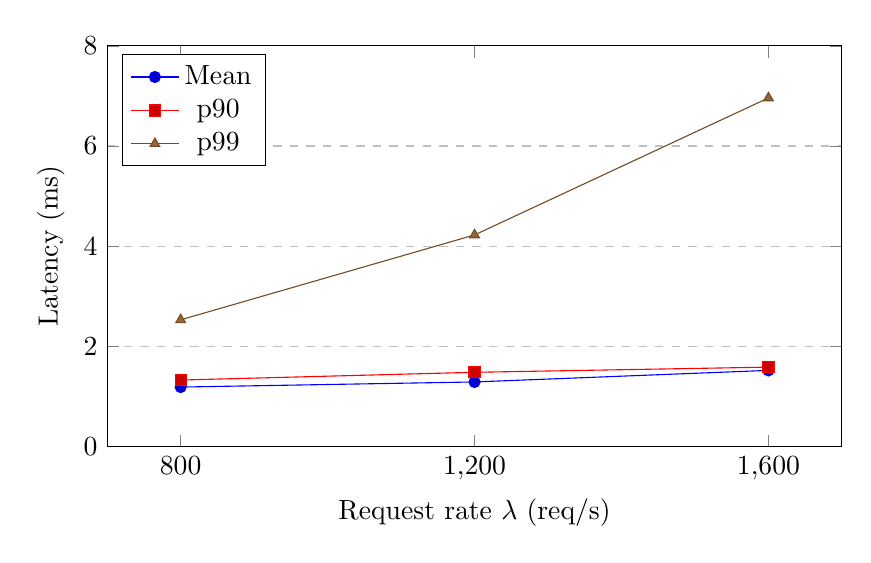
\begin{tikzpicture}
\begin{axis}[
    width=0.9\linewidth,
    height=0.55\linewidth,
    xlabel={Request rate $\lambda$ (req/s)},
    ylabel={Latency (ms)},
    xmin=700, xmax=1700,
    ymin=0, ymax=8,
    xtick={800,1200,1600},
    ymajorgrids=true,
    grid style=dashed,
    legend style={at={(0.02,0.98)},anchor=north west},
]
\addplot+[mark=*] coordinates {
    (800, 1.185)
    (1200, 1.287)
    (1600, 1.518)
};
\addlegendentry{Mean}

\addplot+[mark=square*] coordinates {
    (800, 1.325)
    (1200, 1.480)
    (1600, 1.583)
};
\addlegendentry{p90}

\addplot+[mark=triangle*] coordinates {
    (800, 2.528)
    (1200, 4.223)
    (1600, 6.959)
};
\addlegendentry{p99}
\end{axis}
\end{tikzpicture}
\caption{Mean, p90, and p99 latency versus request rate for the
Dockerised microservice.}
\label{fig:latency-vs-load}
\end{figure}

The figure highlights that the mean and p90 latencies grow slowly with
increasing load, whereas p99 exhibits a much steeper, near-linear
increase across the tested region. In later experiments, higher loads
and reduced CPU quotas are expected to produce the ``latency cliffs''
reported in production systems when utilisation approaches~1.

%-------------------------------------------------------------
\section{Queueing-Theoretic Interpretation}
\label{sec:prelim-qt}

The empirical results can be interpreted through the lens of basic
queueing theory. Let $\lambda$ denote the request rate and $S$ the mean
service time. For a single-server system, the utilisation is
$\rho = \lambda S$, and the classical M/M/1 response-time formula is

\[
  R = \frac{S}{1 - \rho}.
\]

In these preliminary experiments, the effective service time $S$ is not
known a priori, but the low mean latencies (around 1--1.5~ms) suggest
that the system is capable of serving on the order of $10^3$ requests
per second per core. As the offered load increases from 800 to
1600~req/s, the mean latency grows only slightly, which is consistent
with the system approaching, but not yet vastly exceeding, its service
capacity.

However, the p99 and maximum latencies deviate substantially from what an
exponential service-time assumption would predict. Even when the mean
latency remains almost flat, the p99 increases from 2.5~ms to nearly
7~ms, and the maximum latency spikes to almost 100~ms at 1600~req/s.
This behaviour indicates that:

\begin{itemize}
    \item the response-time distribution is not well captured by an exponential
          assumption, as extreme latencies grow disproportionately with load;
    \item contention effects such as CPU saturation and scheduling delays
          produce infrequent but very slow requests; and
    \item purely analytical M/M/1-style models are insufficient for capturing
          extreme-latency behaviour, even if they approximate mean performance
          reasonably well.
\end{itemize}

Direct measurement of CPU throttling and service-time distributions will be
conducted in Thesis~B to determine whether tail latency follows a heavy-tailed
decay pattern or arises primarily from resource contention effects.

These observations align closely with reports from large-scale microservice
deployments, where mean latency can appear healthy while p95/p99 explode near
saturation. This behaviour reinforces why ML is needed to learn the empirical
service-time distribution \(G\) required for the DES model.


%-------------------------------------------------------------
\section{Implications for the Thesis Aims}
\label{sec:prelim-implications}

The experiments above directly support the overall research direction
outlined in Chapters~1--3. The thesis aims to tackle the problem of
predicting service latency, tail behaviour, and saturation thresholds
for containerised microservices under varying load and resource
constraints, using a hybrid DES--ML modelling framework.

The preliminary results demonstrate that:

\begin{enumerate}
    \item \textbf{A single Dockerised microservice exhibits realistic
    capacity-planning phenomena.} Even with a simple echo server, the
    system shows increasing mean latency, sharp growth in p99, and rare
    extreme delays as the request rate rises. This validates Docker as a
    suitable platform for studying microservice performance in a
    controlled educational environment.

    \item \textbf{Empirical traces are rich enough to drive modelling.}
    For each load level, Vegeta provides the full latency distribution,
    while cAdvisor and Prometheus (not tabulated here) provide CPU
    utilisation and throttling metrics. Together, these traces supply
    the arrival rates, service-time samples, and utilisation patterns
    required to parameterise discrete-event simulations and to train
    machine-learning models.

    \item \textbf{Queueing theory alone cannot explain tail behaviour.}
    The heavy-tailed p99 and maximum latencies, despite modest changes
    in mean latency, indicate that exponential assumptions are invalid.
    This confirms the need for ML-based distribution learning (e.g.,
    kernel density estimation, mixture models, or regressors that map
    CPU quotas to service-time parameters) as proposed in the hybrid
    ML--DES framework.

    \item \textbf{The platform is compatible with teaching objectives.}
    All experiments were run on a single student-grade machine using
    Docker, Vegeta, and the Prometheus--Grafana stack. This supports the
    thesis goal of developing a platform that COMP9334 students can run
    locally to compare theoretical predictions from queueing theory and
    DES with real container behaviour.
\end{enumerate}

In summary, the preliminary preparation phase confirms that the proposed
Docker-based environment can (i) reproduce the saturation and tail
phenomena discussed in the literature, and (ii) generate the empirical
traces needed for the hybrid ML--DES modelling pipeline. 
The present evaluation focuses on latency- and load-based measurements, which are sufficient to calibrate the initial discrete-event simulation model. However, contemporary SRE and capacity-planning practice routinely observes additional production metrics—such as CPU throttling, request queue depth, and error-budget burn rates—to understand saturation mechanisms in containerised systems. These metrics require integration with operating-system cgroup counters and service-level objective tracking, which will be incorporated during Thesis~B when the hybrid ML--DES model is developed. At that stage, CPU throttling traces and queue-depth telemetry will be used to refine the service-time models, while error-budget burn will provide an SLO-oriented interpretation of tail latency. Their mention in Chapter~3 therefore reflects industry relevance rather than an omission in the current experimental stage.
Chapter~5
builds on this foundation by outlining the full project plan for
constructing the modelling framework and integrating it into a teaching
tool for capacity planning.

\section{Threats to validity}

Docker Desktop introduces variability due to host OS scheduling and the additional virtualization layer, which can affect fine-grained timing behaviour. Network-stack jitter and the scrape-interval limitations of Prometheus reduce temporal resolution and may mask transient effects. Furthermore, CPU throttling granularity imposed by cgroups can introduce timing artefacts near saturation points. To mitigate these issues, experiments were executed under minimal background load, CPU cores were pinned using --cpuset-cpus, and each measurement was repeated multiple times with averaged results and confidence intervals computed. These mitigations reduce but do not eliminate variance; therefore, all measurements should be interpreted as representative rather than absolute.